\subsection{Misura della capacità di pilotaggio}

\begin{wrapfigure}[14]{l}{0.55\textwidth}
  \begin{center}
    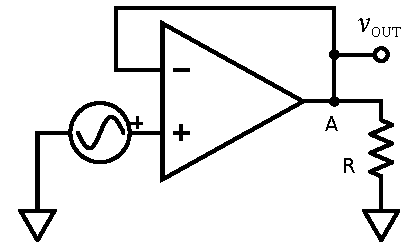
\includegraphics[width=0.26\textwidth]{../E03/latex/max_current.pdf}
  \end{center}
  \caption{Schema del circuito utilizzato per misurare la corrente massima. La resistenza utilizzata è $R=98.47\pm0.01$\si{\ohm}.}
  \label{cir3:max_current}
\end{wrapfigure}

L'amplificatore operazionale ha un valore massimo di corrente erogabile in uscita. Dunque, se montiamo un circuito di feedback come in Figura \ref{cir3:max_current}, la tensione massima ai capi di $R$ sarà fissata dalla corrente massima e dalla resistenza stessa dalla legge di Ohm

$$I_{max} = \frac{V_{clip}}{R}$$

dove $V_{clip}$ è la tensione in cui il segnale in uscita risulta tagliato rispetto a quello in ingresso (fenomeno del \textit{clipping}).

Per misurare $I_{max}$ abbiamo dunque sfruttato questo fatto, ponendo una resistenza di carico fra l'uscita dell'operazionale e terra \footnote{Si noti che, data l'alta impedenza in ingresso dell'oscilloscopio ($1$ \si{\mega\ohm}), non era possibile misurare la corrente massima con questo strumento (attesa, come da specifiche del costruttore, sui $15$ \si{\milli\ampere}): sarebbe servita una tensione di $15000$ \si{\volt}!}, con l'oscilloscopio ai capi di tale resistenza per la misura di tensione (circuito in Figura \ref{cir3:max_current}).

Bisogna però considerare che la corrente, ponendo il segnale in entrata in alternata, risulta oscillare fra valori negativi e positivi (corrente rispettivamente entrante o uscente dal punto A). Inoltre, tali valori sono differenti (si nota dal grafico in Figura ?????? l'asimmetria della tensione di clip):

$$I_{V^+} = \frac{0.9625 \si{\volt}}{R} = 9.8 \si{\milli\volt}  \qquad I_{V^-} = \frac{1.7250 \si{\volt}}{R} = 17.5 \si{\milli\volt}$$

ATTENZIONE! SONO IL DOPPIO + ERRORI!